\documentclass[tikz,border=10pt]{standalone}
\usepackage{amsmath,amssymb}
\usepackage{tikz}
\usetikzlibrary{arrows.meta,positioning,calc,fit,backgrounds}

%% ---- Colour palette (matching overview_arr_clean style) ----
\definecolor{cBlue}{RGB}{200,220,245}
\definecolor{cGreen}{RGB}{200,235,200}
\definecolor{cYellow}{RGB}{255,230,180}
\definecolor{cPink}{RGB}{250,200,200}
\definecolor{cPurple}{RGB}{225,215,245}
\definecolor{cGray}{RGB}{230,230,230}

%% ---- Styles ----
\tikzset{
  basenode/.style={draw, rounded corners=4pt, minimum height=0.7cm,
                   inner sep=4pt, font=\small\sffamily, align=center,
                   line width=0.6pt},
  panel/.style={draw, rounded corners=6pt, thick, inner sep=10pt},
  ptitle/.style={font=\small\sffamily\bfseries, align=center},
  box/.style={basenode, minimum width=1.5cm},
  note/.style={font=\footnotesize\sffamily, inner sep=1pt, align=center},
  smallnote/.style={font=\scriptsize\sffamily, inner sep=1pt, align=left, text=black!70},
  mathnote/.style={font=\footnotesize, inner sep=1pt, align=center},
  myarrow/.style={-{Stealth[length=5pt]}, thick},
  dashbox/.style={draw, dashed, rounded corners=4pt, line width=0.5pt,
                  inner sep=5pt, font=\scriptsize\sffamily, align=left},
  explain/.style={font=\scriptsize\sffamily, text=black!65, align=left, inner sep=1pt},
  bulnote/.style={font=\scriptsize\sffamily, text=black!70, inner sep=0pt},
}

\begin{document}
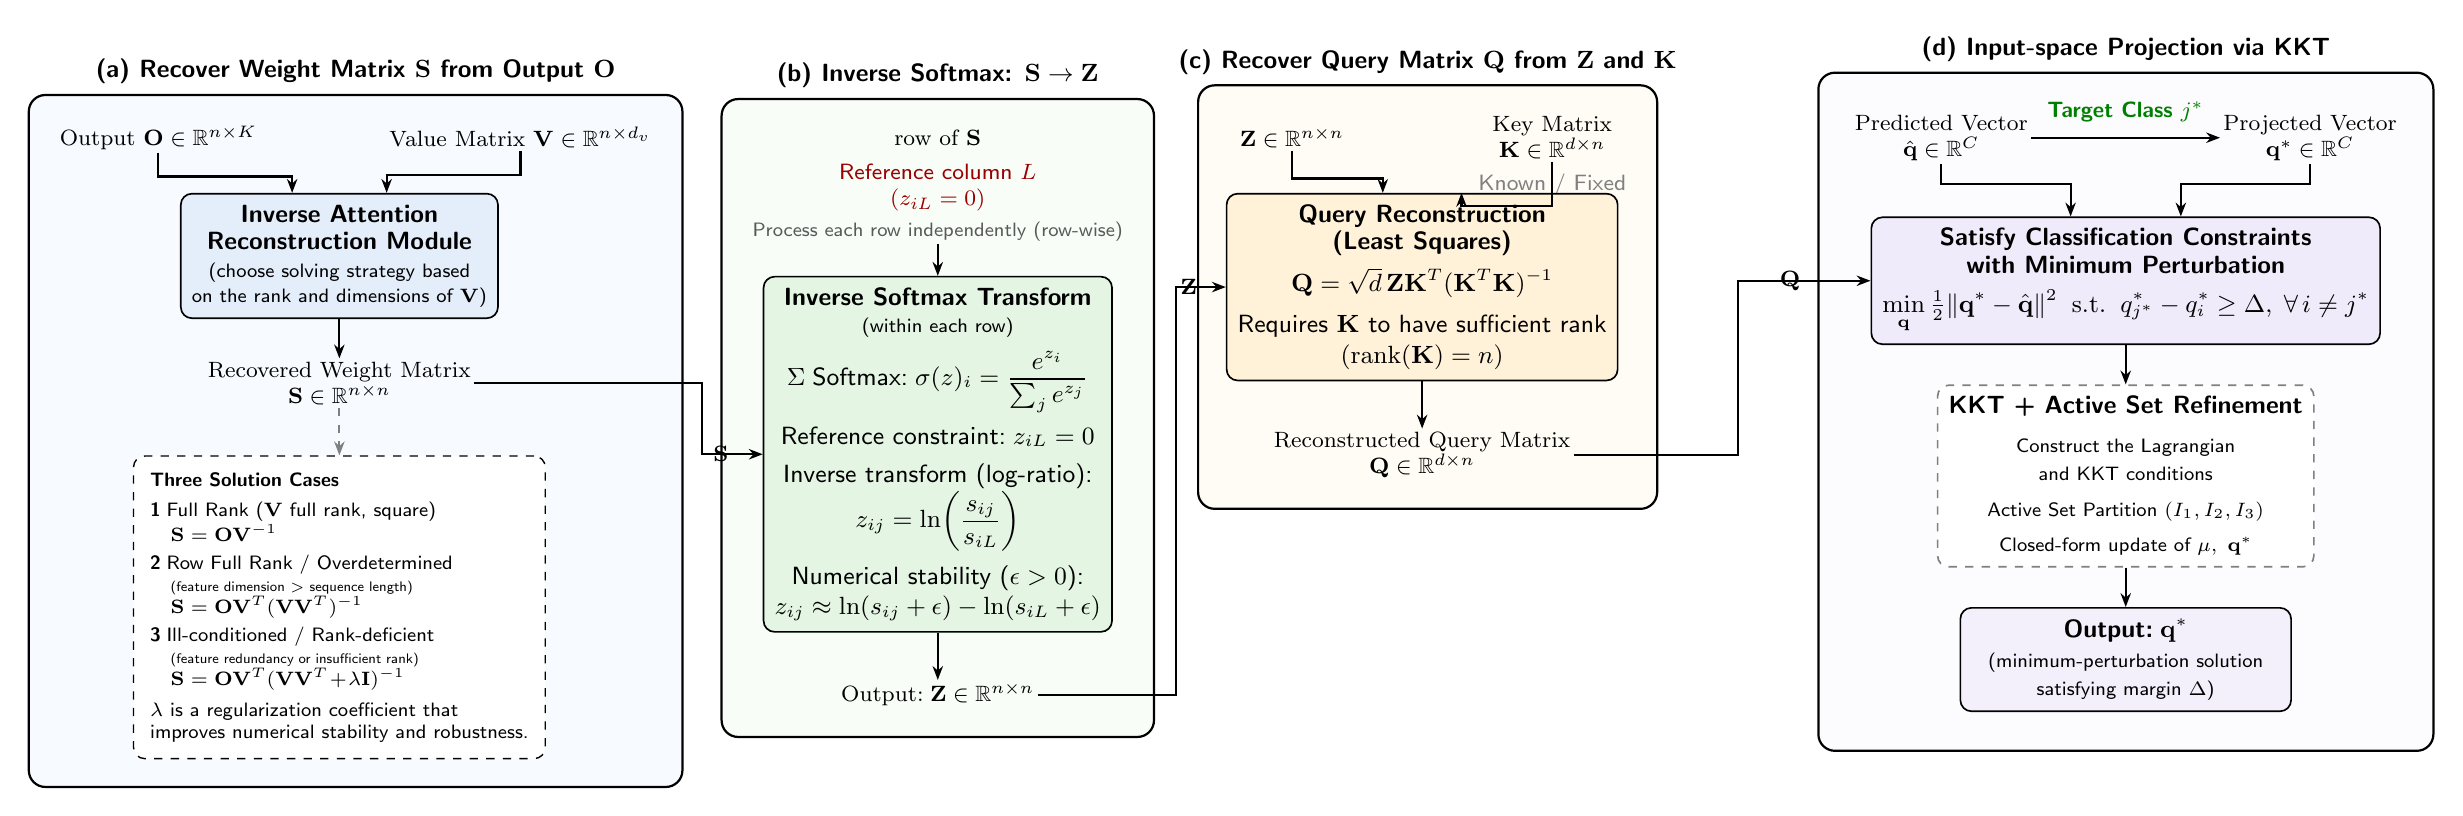
\begin{tikzpicture}[node distance=0.55cm and 0.6cm]

%% ================================================================
%%  (a) Recover S from O
%% ================================================================

\node[mathnote] (Olabel) at (0, 11.2) {Output $\mathbf{O}\in\mathbb{R}^{n\times K}$};
\node[mathnote, right=1.6cm of Olabel] (Vlabel) {Value Matrix $\mathbf{V}\in\mathbb{R}^{n\times d_v}$};

\node[box, fill=cBlue!50, minimum width=3.4cm, minimum height=1.1cm,
      below=0.7cm of $(Olabel)!0.5!(Vlabel)$] (solver)
  {\textbf{Inverse Attention}\\[-1pt]\textbf{Reconstruction Module}\\[-1pt]
   {\scriptsize (choose solving strategy based}\\[-2pt]
   {\scriptsize on the rank and dimensions of $\mathbf{V}$)}};

\draw[myarrow] (Olabel.south) -- ++(0,-0.3) -| ([xshift=-0.6cm]solver.north);
\draw[myarrow] (Vlabel.south) -- ++(0,-0.3) -| ([xshift=0.6cm]solver.north);

%% Recovered S output
\node[mathnote, below=0.5cm of solver] (Stext) {Recovered Weight Matrix\\$\mathbf{S}\in\mathbb{R}^{n\times n}$};
\draw[myarrow] (solver) -- (Stext);

%% Three Solution Cases box with explanations
\node[dashbox, fill=white, below=0.6cm of Stext, minimum width=3.8cm, inner sep=6pt] (cases)
  {\textbf{Three Solution Cases}\\[3pt]
   \textbf{1}\;Full Rank ($\mathbf{V}$ full rank, square)\\
   \quad $\mathbf{S}=\mathbf{O}\mathbf{V}^{-1}$\\[2pt]
   \textbf{2}\;Row Full Rank / Overdetermined\\
   \quad{\tiny (feature dimension $>$ sequence length)}\\
   \quad $\mathbf{S}=\mathbf{O}\mathbf{V}^{T}(\mathbf{V}\mathbf{V}^{T})^{-1}$\\[2pt]
   \textbf{3}\;Ill-conditioned / Rank-deficient\\
   \quad{\tiny (feature redundancy or insufficient rank)}\\
   \quad $\mathbf{S}=\mathbf{O}\mathbf{V}^{T}(\mathbf{V}\mathbf{V}^{T}\!+\!\lambda\mathbf{I})^{-1}$\\[3pt]
   $\lambda$ is a regularization coefficient that\\
   improves numerical stability and robustness.};
\draw[myarrow, dashed, gray] (Stext) -- (cases);

\begin{scope}[on background layer]
  \node[panel, fill=cBlue!15, fit=(Olabel)(Vlabel)(solver)(Stext)(cases),
        label={[ptitle]above:\textbf{(a) Recover Weight Matrix $\mathbf{S}$ from Output $\mathbf{O}$}}] (panelA) {};
\end{scope}

%% ================================================================
%%  (b) Inverse Softmax
%% ================================================================

\node[mathnote, right=2.2cm of Vlabel, xshift=0.8cm] (rowS) {row of $\mathbf{S}$};
\node[note, below=0.15cm of rowS, text=red!60!black] (refcol)
  {Reference column $L$\\$(z_{iL}=0)$};
\node[explain, below=0.05cm of refcol] (rowexp) {Process each row independently (row-wise)};

\node[box, fill=cGreen!50, minimum width=3.6cm, minimum height=2.6cm,
      below=0.4cm of rowexp] (invsoft)
  {\textbf{Inverse Softmax Transform}\\[-1pt]{\scriptsize (within each row)}\\[4pt]
   $\Sigma$\;Softmax:\;$\displaystyle\sigma(z)_i=\frac{e^{z_i}}{\sum_j e^{z_j}}$\\[4pt]
   Reference constraint:\;$z_{iL}=0$\\[3pt]
   Inverse transform (log-ratio):\\
   $\displaystyle z_{ij}=\ln\!\left(\frac{s_{ij}}{s_{iL}}\right)$\\[4pt]
   Numerical stability ($\epsilon>0$):\\
   $z_{ij}\approx\ln(s_{ij}+\epsilon)-\ln(s_{iL}+\epsilon)$};

\draw[myarrow] (rowexp.south) -- (invsoft.north);

\node[mathnote, below=0.6cm of invsoft] (Ztext) {Output:\;$\mathbf{Z}\in\mathbb{R}^{n\times n}$};
\draw[myarrow] (invsoft) -- (Ztext);

\begin{scope}[on background layer]
  \node[panel, fill=cGreen!12, fit=(rowS)(refcol)(rowexp)(invsoft)(Ztext),
        label={[ptitle]above:\textbf{(b) Inverse Softmax: $\mathbf{S}\rightarrow\mathbf{Z}$}}] (panelB) {};
\end{scope}

%% ================================================================
%%  (c) Recover Q from Z and K
%% ================================================================

\node[mathnote, right=2.2cm of rowS, xshift=1.0cm] (Zlabel) {$\mathbf{Z}\in\mathbb{R}^{n\times n}$};
\node[mathnote, right=1.8cm of Zlabel] (Klabel) {Key Matrix\\$\mathbf{K}\in\mathbb{R}^{d\times n}$};
\node[note, below=0.1cm of Klabel, text=gray] (known) {Known / Fixed};

\node[box, fill=cYellow!50, minimum width=3.4cm, minimum height=1.8cm,
      below=0.7cm of $(Zlabel)!0.5!(Klabel)$] (lsq)
  {\textbf{Query Reconstruction}\\[-1pt]\textbf{(Least Squares)}\\[4pt]
   $\mathbf{Q}=\sqrt{d}\,\mathbf{Z}\mathbf{K}^{T}(\mathbf{K}^{T}\mathbf{K})^{-1}$\\[4pt]
   Requires $\mathbf{K}$ to have sufficient rank\\
   $(\operatorname{rank}(\mathbf{K})=n)$};

\draw[myarrow] (Zlabel.south) -- ++(0,-0.35) -| ([xshift=-0.5cm]lsq.north);
\draw[myarrow] (Klabel.south) -- ++(0,-0.55) -| ([xshift=0.5cm]lsq.north);

\node[mathnote, below=0.6cm of lsq] (Qtext) {Reconstructed Query Matrix\\$\mathbf{Q}\in\mathbb{R}^{d\times n}$};
\draw[myarrow] (lsq) -- (Qtext);

\begin{scope}[on background layer]
  \node[panel, fill=cYellow!12, fit=(Zlabel)(Klabel)(known)(lsq)(Qtext),
        label={[ptitle]above:\textbf{(c) Recover Query Matrix $\mathbf{Q}$ from $\mathbf{Z}$ and $\mathbf{K}$}}] (panelC) {};
\end{scope}

%% ================================================================
%%  (d) Input-space Projection via KKT
%% ================================================================

\node[mathnote, right=2.2cm of Klabel, xshift=0.8cm] (qhat) {Predicted Vector\\$\hat{\mathbf{q}}\in\mathbb{R}^{C}$};
\node[mathnote, right=2.4cm of qhat] (qstar) {Projected Vector\\$\mathbf{q}^{*}\in\mathbb{R}^{C}$};

%% Arrow qhat -> qstar
\draw[myarrow] (qhat.east) -- (qstar.west)
  node[pos=0.5, above=0.15cm, note, text=green!50!black, font=\footnotesize\sffamily\bfseries] {Target Class $j^{*}$};

%% Satisfy constraints box
\node[box, fill=cPurple!50, minimum width=4.4cm, minimum height=1.0cm,
      below=1.0cm of $(qhat)!0.5!(qstar)$] (cons)
  {\textbf{Satisfy Classification Constraints}\\[-1pt]\textbf{with Minimum Perturbation}\\[3pt]
   $\displaystyle\min_{\mathbf{q}}\tfrac{1}{2}\|\mathbf{q}^{*}-\hat{\mathbf{q}}\|^2
    \;\;\mathrm{s.t.}\;\;q^{*}_{j^{*}}-q^{*}_{i}\ge\Delta,\;\forall\,i\ne j^{*}$};

\draw[myarrow] (qhat.south) -- ++(0,-0.25) -| ([xshift=-0.7cm]cons.north);
\draw[myarrow] (qstar.south) -- ++(0,-0.25) -| ([xshift=0.7cm]cons.north);

%% KKT box with three-step explanation
\node[box, fill=white, draw=gray, dashed, minimum width=4.4cm, minimum height=1.2cm,
      below=0.5cm of cons] (kkt)
  {\textbf{KKT + Active Set Refinement}\\[3pt]
   {\scriptsize Construct the Lagrangian}\\[-1pt]
   {\scriptsize and KKT conditions}\\[2pt]
   {\scriptsize Active Set Partition $(I_1,I_2,I_3)$}\\[2pt]
   {\scriptsize Closed-form update of $\mu,\;\mathbf{q}^{*}$}};
\draw[myarrow] (cons) -- (kkt);

%% Output with description
\node[box, fill=cPurple!40, minimum width=4.2cm, below=0.5cm of kkt] (outq)
  {\textbf{Output:}\;$\mathbf{q}^{*}$\\{\scriptsize (minimum-perturbation solution}\\[-1pt]
   {\scriptsize satisfying margin $\Delta$)}};
\draw[myarrow] (kkt) -- (outq);

\begin{scope}[on background layer]
  \node[panel, fill=cPurple!10, fit=(qhat)(qstar)(cons)(kkt)(outq),
        inner ysep=14pt, inner xsep=12pt,
        label={[ptitle]above:\textbf{(d) Input-space Projection via KKT}}] (panelD) {};
\end{scope}

%% ================================================================
%%  Inter-panel arrows
%% ================================================================

\coordinate (midAB) at ($(panelA.east)!0.5!(panelB.west)$);
\draw[myarrow, thick]
  (Stext.east) -- (midAB |- Stext.east)
  -- (midAB |- invsoft.west)
  -- (invsoft.west)
  node[pos=0.5, left, note] {$\mathbf{S}$};

\coordinate (midBC) at ($(panelB.east)!0.5!(panelC.west)$);
\draw[myarrow, thick]
  (Ztext.east) -- (midBC |- Ztext.east)
  -- (midBC |- lsq.west)
  -- (lsq.west)
  node[pos=0.5, left, note] {$\mathbf{Z}$};

\coordinate (midCD) at ($(panelC.east)!0.5!(panelD.west)$);
\draw[myarrow, thick]
  (Qtext.east) -- (midCD |- Qtext.east)
  -- (midCD |- cons.west)
  -- (cons.west)
  node[pos=0.5, left, note] {$\mathbf{Q}$};

\end{tikzpicture}
\end{document}
